\documentclass[letterpaper,12pt]{article}
\usepackage{tabularx} % extra features for tabular environment
\usepackage{amsmath}  % improve math presentation
\usepackage{graphicx, subcaption} % takes care of graphic including machinery
\usepackage[margin=1in,letterpaper]{geometry} % decreases margins
\usepackage{xspace}
\usepackage{ANA-FTAG-2020-08-PAPER-defs}
\usepackage[style=numeric, sorting=none]{biblatex}
\addbibresource{ANA-FTAG-2020-08-PAPER.bib}
\addbibresource{bib/ATLAS.bib}
\addbibresource{bib/ATLAS-useful.bib}
\addbibresource{bib/PubNotes.bib}
\addbibresource{bib/ConfNotes.bib}
\addbibresource{bib/ATLAS-SUSY.bib}

\usepackage[final]{hyperref} % adds hyper links inside the generated pdf file
\usepackage[T1]{fontenc}
\usepackage{setspace}
\usepackage{float}
\usepackage{makeidx}
\usepackage{titlesec}

\newcommand\bjetineq{\mathop{\mbox{$b$ $\rm{jet}$}}}
\newcommand\bjetunder{\mathop{\footnotesize{\mbox{$b$ $\rm{jet}$}}}\normalsize}
\newcommand\cjetineq{\mathop{\mbox{$c$ $\rm{jet}$}}}
\newcommand\cjetunder{\mathop{\footnotesize{\mbox{$c$ $\rm{jet}$}}}\normalsize}
\setcounter{secnumdepth}{4}
\newcommand{\specialcell}[2][c]{%
  \begin{tabular}[#1]{@{}c@{}}#2\end{tabular}}

\titleformat{\paragraph}
{\normalfont\normalsize\bfseries}{\theparagraph}{1em}{}
\titlespacing*{\paragraph}
{0pt}{3.25ex plus 1ex minus .2ex}{1.5ex plus .2ex}
\restylefloat*{figure}
\hypersetup{
	colorlinks=true,       % false: boxed links; true: colored links
	linkcolor=blue,        % color of internal links
	citecolor=blue,        % color of links to bibliography
	filecolor=magenta,     % color of file links
	urlcolor=blue         
}

%++++++++++++++++++++++++++++++++++++++++
\linespread{1.17}
\makeindex
\begin{document}


\title{Search for Higgs boson pair-production in the $bb\tau\tau$ final state using proton-proton collisions at $\sqrt{s}$ = 13 \TeV\ data with the ATLAS detector}%Fake Factors Calculation and Implementation in H$\rightarrow$ bb$\tau^+\tau^-$ analysis with MC16a/MC16d in Release 21 with the ATLAS detector
\author{ Zhiyuan Li}
\date{\today}
\maketitle
\begin{figure}[htp]
\centering

\includegraphics[width=.5\textwidth]{logo.png}
\vspace{3em}
\centering

\includegraphics[width=.45\textwidth]{ATLAS-Logo-Ref-RGB-H_1.jpg}
\end{figure}
\newpage


\tableofcontents{}
\printindex{}


\newpage
\section{Introduction}
\section{Theory and Motivation}
\subsection{The Standard Model and the Higgs boson}
\subsection{Beyond the Standard Model}
\section{The ATLAS experiment at the Large Hadron Collider}
\subsection{The Large Hadron Collider}

The Large Hadron Collider [cite{Evans:2008zzb}] is the world's largest and most powerful particle accelerator. 
It started in 2008 and remains its crucial role in the many accelerators at CERN and in the world.
The main body of the collider consists of a ring tunnel of perimeter of 26.7 km, with 
superconducting magnets along the tunnel to keep the particle beam in direction
 and a large number of accelerating structures to boost the beam to the desired energy.

Inside the tunnel, two beams of particles travelling at close to the speed of light 
in opposite direction are made to collide. These two beams are kept in separate beam pipes,
cooled to $-271.3^\circ C$ ($1.9K$) with liquid helium distributed by dedicated system, 
 and ultra-high vacuum, a vacuum thinner than 
interstellar void, matianed for 48 km of low-temperature section and 6 km of room-temperature 
section. 

Thousands of magnets are used to direct the beams along the beam pipe, either to bend the beams or
to focus. The particles are so small that making them collide is akin to 
firing two needles 10 kilometers away and meet halfway. 

All the controls for the accelerator, its services and technical infrastructure 
are located at the CERN Control Centre. 
From here, the beams inside the LHC are made to collide at four locations around the accelerator ring, 
corresponding to the positions of four particle detectors – ATLAS (A Toroidal LHC ApparatuS) [cite{PERF-2007-01}], 
CMS [S08004] (Compact Muon Solenoid), ALICE (A Large Ion Collider Experiment) [S08002] 
and LHCb (b stands for beauty) [S08005].


	\subsubsection{Design and performance}

	The LHC is a two-ring-superconducting-hadron accelerator and collider
	installed in the existing 26.7 km tunnel that was constructed between 1984 and 1989 
	for the CERN LEP machine. The LEP tunnel has eight straight sections and eight arcs 
	and lies between 45 m and 170 m below the surface on a plane inclined at 1.4\% sloping towards the Léman lake.
	Approximately 90\% of its length is in molasse rock, which has excellent characteristics for this application,
	and 10\% is in limestone under the Jura mountain. There are two transfer tunnels, 
	each approxi-mately 2.5 km in length, linking the LHC to the CERN accelerator complex that acts as injector.
	As mentioned before, the beam piples are maintained in vacuum for low and high temperature section.
	For the low temperature section, the vacuum is achieved by pumping in 9000 $m^3$ of cryogenic
	gas, which later will be condensed and adhered to the surface of the beampipe. For the room temperature
	section, the vacuum is achieved by use of non-evaporable getter (NEG) that absorbs residue gas particles 
	when heated. More residue is absorbed by ion pumper. 

	Being a proton-proton (pp) collider, there are advantages and disadvantages compared to a
	proton-anti-proton collider and an electron-positron collider. 
	Two rings are needed to accommodate the two counter-rotatign beams, unlike particle-antiparticle 
	colliders that can have both beams sharing the same phase space in a single ring.
	However it would not be possible to to achieve such high luminosity using
	anti-proton beams. 
	In principle, the mass of the proton is much larger than the mass of the electron, the
	synchrotron radiation losses will be much smaller, and the long straight sections designed for
	compensate the losses (as designed in the LEP) can be reduced. However these sections are kept 
	as the LEP has as a cost-effective solution. 
	The tunnel in the arcs has a finished internal diameter of 3.7 m, 
	due to the technical difficulties to install two separate rings in such small space,
	
	It was proposed by John Blewett at the Brookhaven laboratory in 1971 first for
	cost consideration [J.P. Blewett, 200GeV intersecting storage accelerators,Proceedings of the8thInternationalConference on High-Energy Accelerators, CERN, Geneva Switzerland (1971)],
	but in the case of the LHC the overriding reason for adopting this solution
	is the lack of space in the tunnel. 
    
    
The ATLAS Collaboration uses various algorithms to identify 
\bjets \cite{PERF-2012-04}, referred to as \btagging\ algorithms, 
when analysing data recorded during Run 2 of the LHC. These 
algorithms exploit the long lifetime, high mass and high decay 
multiplicity of $b$-hadrons, as well as the properties of the \bquark\  
fragmentation. Given a lifetime of the order of 1.5 ps, $b$-hadrons have a 
significant mean flight length ($\langle c\tau \rangle$ $\approx$ 450 $\mu m$), 
in the detector before decaying, generally leading to at least one vertex 
displaced from the hard-scatter collision point, as illustrated in Figure~\ref{fig:b-jet-decay}.

\begin{figure}[]
	\begin{centering}	
	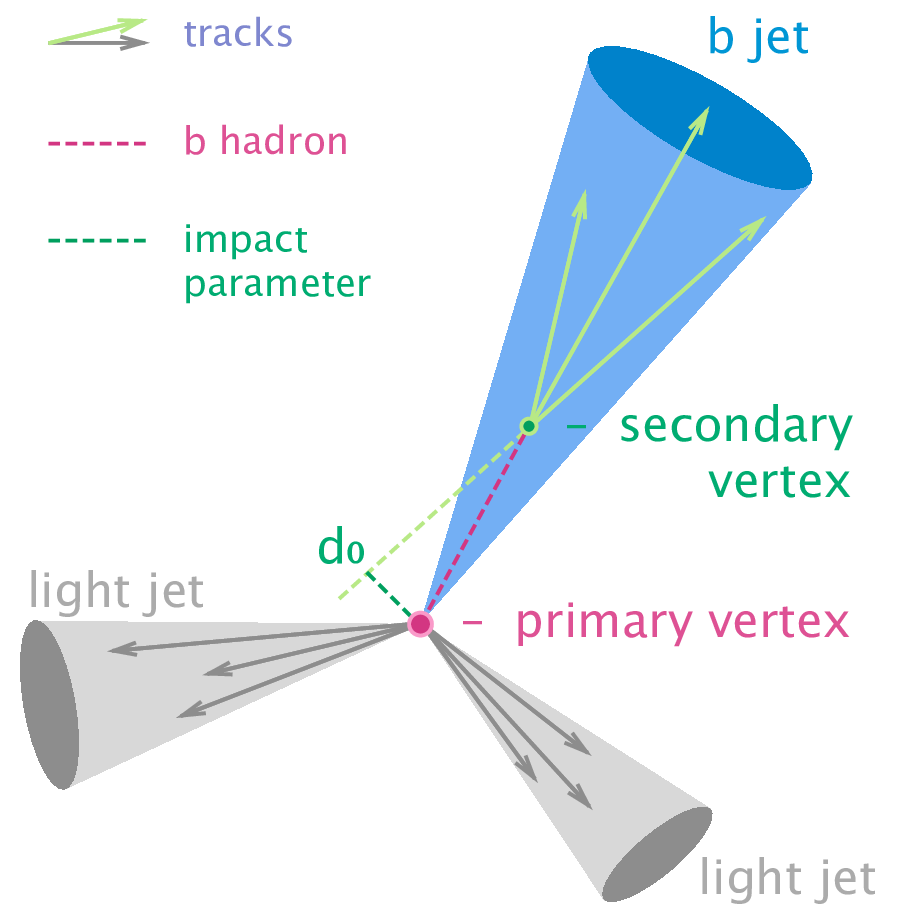
\includegraphics[width=.4\textwidth]{FTAG_plots/B-tagging_diagram.png}
	\caption{A diagram showning the b hadron decay initiated jets. }
	\label{fig:b-jet-decay}
	\end{centering}
\end{figure}


\begin{figure}[]
    \begin{centering}	
    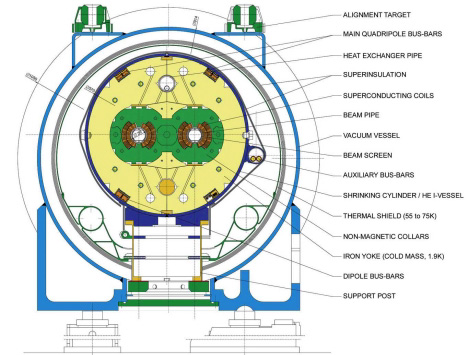
\includegraphics[width=.4\textwidth]{Detector_plots/LHC-double-bore-magnet.jpg}
    \caption{ Double-bore magnet configuration of the LHC superconducting magnets.[THE LHC SUPERCONDUCTING MAGNETSL. Rossi, Accelerator Technology Division, CERN, Geneva, Switzerland]
        }
    \label{fig:double-bore-magnet}
    \end{centering}
\end{figure}

\end{document}